%%%_* Document preamble
\documentclass[14pt,t,usepdftitle=false,
xcolornames=x11names,svgnames,dvipsnames]{beamer}
\usepackage{fontspec}
\usepackage{listings}
\usepackage{alltt}
\usepackage{mathptmx}
\usepackage{times}
%%%_* Simplest theme ever; white background, no widgets
\usetheme{default}
\setbeamertemplate{navigation symbols}{}
\setbeameroption{show notes}
\setbeamertemplate{frametitle}[default][center]
\setbeamersize{text margin left=10mm}
%%%_** Fancy fonts
\setbeamerfont{frametitle}{series=\bfseries}
\setmainfont[Mapping=tex-text]{Warnock Pro}
\setsansfont[Mapping=tex-text,Numbers={OldStyle}]{Cronos Pro}
\setmonofont[Mapping=tex-text]{Inconsolata}
\newcommand{\wackyFont}[1]{
  {\huge\fontspec[Mapping=tex-text]{Immi Five O Five Std} #1}}
\newcommand{\subtitleFont}[1]{{\footnotesize #1}}
\newcommand{\slideheading}[1]{
  \begin{center}
    \usebeamerfont{frametitle}
    \usebeamercolor[fg]{frametitle}#1
  \end{center}\vskip-5mm}
\usefonttheme{professionalfonts}
%%%_** Font samples
\newcommand{\foreachFontA}[1]{
  #1{Adobe Caslon Pro} #1{Adobe Garamond Pro} #1{Adobe Jenson Pro}
  #1{Arno Pro}         #1{Bell Gothic Std}    #1{Century Old Style Std}
  #1{Chaparral Pro}    #1{Conga Brava Std}}
\newcommand{\foreachFontB}[1]{
  #1{Cronos Pro}       #1{Garamond Premier Pro} #1{Immi Five O Five Std}
  #1{Minion Pro}       #1{Myriad Pro}           #1{Nueva Std}
  #1{Tekton Pro}       #1{Warnock Pro}}
\newcommand{\foreachFontM}[1]{
  #1{Inconsolata} #1{Letter Gothic Std} #1{Prestige Elite Std}}
\newcommand{\fontSampleF}[3]{
  #1 #3 123abcgyqz fi fl ffi \textbf{bold} \textit{italic}
  #2 123\\}
\newcommand{\fontSample}[1]{
  \fontSampleF{\fontspec{#1}}{\fontspec[Numbers={OldStyle}]{#1}}{#1}}
\newcommand{\fontSamples}{      %%%
  \frame{\foreachFontA{\fontSample}}
  \frame{\foreachFontB{\fontSample}}
  \frame{\fontfamily{lmtt}\selectfont
    \fontSampleF{\relax}{\relax}{Computer Modern Typewriter}
    \foreachFontM{\fontSample}}}

%%%_** Color definitions
\colorlet{comment}{Olive}
\colorlet{string}{SaddleBrown}
\colorlet{keyword}{Navy}
\colorlet{type}{Green}
\colorlet{emph}{Maroon}
\colorlet{input}{Indigo}
\colorlet{error}{DarkRed}
\colorlet{result}{LightSlateGrey}
\colorlet{background}{LightGoldenrodYellow}
\colorlet{hole}{LimeGreen}

%%%_** Listings settings
% "define" Scala
\lstdefinelanguage{scala}{
  morekeywords={abstract,case,catch,class,def,%
    do,else,extends,false,final,finally,%
    for,if,implicit,import,match,mixin,%
    new,null,object,override,package,%
    private,protected,requires,return,sealed,%
    super,this,throw,trait,true,try,%
    type,val,var,while,with,yield},
  otherkeywords={=,=>,<-,<\%,<:,>:,\#,@},
  emph={String,Int,Boolean,Unit,Float,Any,Double,List},
  sensitive=true,
  morecomment=[l]{//},
  morecomment=[n]{/*}{*/},
  morestring=[b]",
  morestring=[b]',
  morestring=[b]"""
}
\lstdefinestyle{scala}{
  language=scala,
  numbers=none,
  numberstyle=\tiny, 
  numbersep=5pt,
  delim=[is][\color{hole}\colorbox{hole}]{(/)}{(/)},
}
\lstdefinestyle{scalarepl}{
  language=scala,
  moredelim=[l][\color{input}]{scala>},
  moredelim=[l][\color{result}]{res},
  frame=single,
  backgroundcolor={\color{background}},
}
\lstdefinestyle{smlrepl}{
  moredelim=[l][\color{input}]{- },
  moredelim=[l][\color{result}]{val },
  moredelim=[l][\color{error}]{uncaught},
  moredelim=[l][\color{error}]{raised},
  moredelim=[s][\color{emph}]{\[}{\]}
}
\lstset{
  columns=flexible,
  showstringspaces=false,
  basicstyle={\small\ttfamily},
  keywordstyle={\bfseries\color{keyword}},
  commentstyle=\color{comment},
  stringstyle=\color{string},
  emphstyle={\color{type}},
  emphstyle={[2]\color{emph}},
  breakatwhitespace=true,
  tabsize=3,
}

%%%_* Metadata
\title{\wackyFont{Continuations}}
\subtitle{\textbf{and other Functional Patterns}}
\author{Christopher League\\\subtitleFont{Long Island University}}
\date{\subtitleFont{Northeast Scala Symposium\\18 February 2011}}
%%%_* Document
\begin{document}
\maketitle


\begin{frame}
  \frametitle{Sin \& redemption}
  
\includegraphics[scale=.36]{tweet-league}\\
  
\includegraphics[scale=.36]{tweet-jamesiry}\\
  
\includegraphics[scale=.36]{tweet-softprops}
\end{frame}

{\setbeamercolor{background canvas}{bg=black}
\begin{frame}
  \begin{center}
    \vspace*{-30mm}
    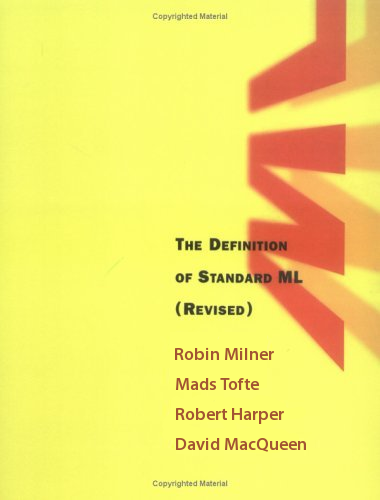
\includegraphics[scale=.72]{sml-book}
  \end{center}
\end{frame}

\begin{frame}
  \vspace*{-10mm}
  \begin{center}
    
\includegraphics[scale=.72]{appel-book}
  \end{center}
\end{frame}
}

\begin{frame}[fragile]{Java classes $\to$ SML runtime}
\begin{lstlisting}[style=smlrepl,basicstyle={\footnotesize\ttfamily}]
 Standard ML of New Jersey v110.30 [JFLINT 1.2]
 - Java.classPath := ["/home/league/r/java/tests"];
 val it = () : unit
 - val main = Java.run "Hello";
 [parsing Hello]
 [parsing java/lang/Object]
 [compiling java/lang/Object]
 [compiling Hello]
 [initializing java/lang/Object]
 [initializing Hello]
 val main = fn : string list -> unit
 - main ["World"];
 Hello, World
 val it = () : unit
 - main [];
 uncaught exception ArrayIndexOutOfBounds
   raised at: Hello.main([Ljava/lang/String;)V
 - ^D
\end{lstlisting}
\end{frame}

\begin{frame}{OO runtime $\leftarrow$ functional languages}
  \begin{center}\large
    \textbf{Scala}\bigskip

    Clojure\bigskip

    F\#\bigskip

    \textit{etc.}
  \end{center}
\end{frame}
%%%%%%%%%%%%%%%%%%%%%%%%%%%%%%%%%%%%%%%%%%%%%%%%%%%%%%%%%%%%
\begin{frame}
    \frametitle{Patterns}
    \begin{enumerate}
    \item Continuation-passing style
    \item Format combinators
    \item Nested data types
    \end{enumerate}
  \slideheading{Theme}
    \begin{itemize}
    \item Higher-order \{functions, types\}
    \end{itemize}
\end{frame}

\begin{frame}
  \frametitle{Pattern 1: Continuations}
  A \textbf{continuation} is an argument that represents\\ the
  \emph{rest} of the computation meant to occur\\after the current
  function.
\end{frame}

\begin{frame}[fragile]
  \frametitle{Explicit continuations -- straight-line}
\begin{lstlisting}[style=scala,moreemph={A}]
  def greeting [A] (name: String) (k: => A): A =
    printk("Hello, ") {
    printk(name) {
    printk("!\n")(k)
    }}
  def printk [A] (s: String) (k: => A): A =
    { Console.print(s); k }
\end{lstlisting}
\begin{lstlisting}[style=scalarepl]
scala> greeting("Scala peeps") { true }
Hello, Scala peeps!
res0: Boolean = true
\end{lstlisting}
\end{frame}

\begin{frame}
  \frametitle{Pay it forward\dots}
  Current function can `return' a value\\by passing it as a
  \textit{parameter} to its continuation.
\end{frame}

\begin{frame}[fragile]
  \frametitle{Explicit continuations -- return values}
\begin{lstlisting}[style=scala,moreemph={A}]
  def plus [A] (x: Int, y: Int) (k: Int => A): A =
    k(x+y)
  def times [A] (x: Int, y: Int) (k: Int => A): A =
    k(x*y)
  def less[A] (x: Int, y: Int) (kt: =>A) (kf: =>A):A =
    if(x < y) kt else kf

  def test[A](k: String => A): A =
    plus(3,2) { a => times(3,2) { b =>
    less(a,b) {k("yes")} {k("no")} }}
\end{lstlisting}
\begin{lstlisting}[style=scalarepl]
scala> test{printk(_){}}
yes
\end{lstlisting}
\end{frame}

\begin{frame}
  \frametitle{Delimited continuations}
  \bigskip
  \begin{description}
  \item[reset] Serves as delimiter for CPS transformation.\medskip
  \item[shift] Captures current continuation as a function\\
    (up to dynamically-enclosing \emph{reset})\\
    then runs specified block instead.
  \end{description}
\end{frame}

\begin{frame}[fragile]
  \frametitle{Delimited continuations}
\begin{lstlisting}[style=scala,emph={[2]reset}]
def doSomething0 = reset {
  println("Ready?")
  val result = 1 + (/)~~~~~~~~(/) * 3
  println(result)
}
\end{lstlisting}

  Think of the \emph{rest} of the computation\\as a \emph{function}
  with the hole as its parameter.
\end{frame}

\begin{frame}[fragile]
  \frametitle{Delimited continuations}
\begin{lstlisting}[style=scala,emph={[2]reset,shift}]
def doSomething1 = reset {
  println("Ready?")
  val result = 1 + special * 3
  println(result)
}
def special = shift {
  k: (Int => Unit) => println(99); "Gotcha!"
}
\end{lstlisting}
  \textit{shift} captures continuation as \textit{k}\\and then determines its
  \textbf{own} future.
\end{frame}

\begin{frame}[fragile]
  \frametitle{Delimited continuations}
\begin{lstlisting}[style=scala,emph={[2]reset,shift}]
def doSomething1 = reset {
  println("Ready?")
  val result = 1 + special * 3
  println(result)
}
def special = shift {
  k: (Int => Unit) => println(99); "Gotcha!"
}
\end{lstlisting}
\begin{lstlisting}[style=scalarepl]
scala> doSomething1
Ready?
99
res0: java.lang.String = Gotcha!
\end{lstlisting}
\end{frame}

\iffalse
\begin{frame}[fragile]
  \frametitle{Delimited continuations}
\begin{lstlisting}[style=scala,emph={[2]reset,shift}]
def doSomething2 = reset {
  println("Ready?")
  val result = 1 + wacky * 3
  println(result)
}
def wacky = shift {
  k: (Int => Unit) => k(2); println("Yo!"); k(3)
}
\end{lstlisting}
\begin{lstlisting}[style=scalarepl]
scala> doSomething2
Ready?
7
Yo!
10
\end{lstlisting}
\end{frame}
\fi

\begin{frame}[fragile]
  \frametitle{Continuation-based user interaction}
\begin{lstlisting}[style=scala,emph={[2]reset,shift}]
def interact = reset {
  val a = ask("Please give me a number")
  val b = ask("Please enter another number")
  printf("The sum of your numbers is: %d\n", a+b)
}
\end{lstlisting}
\begin{lstlisting}[style=scalarepl]
scala> interact
Please give me a number
answer using: submit(0xa9db9535, ...)
scala> submit(0xa9db9535, 14)
Please enter another number
answer using: submit(0xbd1b3eb0, ...)
scala> submit(0xbd1b3eb0, 28)
The sum of your numbers is: 42
\end{lstlisting}
\end{frame}

\begin{frame}[fragile]
  \frametitle{Continuation-based user interaction}
\begin{lstlisting}[style=scala,emph={[2]reset,shift}]
val sessions = new HashMap[UUID, Int=>Unit]
def ask(prompt: String): Int @cps[Unit] = shift {
    k: (Int => Unit) => {
      val id = uuidGen
      printf("%s\nanswer using: submit(0x%x, ...)\n",
             prompt, id)
      sessions += id -> k
  }}
def submit(id: UUID, data: Int) = sessions(id)(data)

def interact = reset {
  val a = ask("Please give me a number")
  val b = ask("Please enter another number")
  printf("The sum of your numbers is: %d\n", a+b)
}
\end{lstlisting}
\end{frame}


%%%%%%%%%%%%%%%%%%%%%%%%%%%%%%%%%%%%%%%%%%%%%%%%%%%%%%%%%%%%

\begin{frame}[fragile]
  \frametitle{Pattern 2: Format combinators}
  \hfill[Danvy 1998]

  Typeful programmers covet \textit{printf}.
\begin{lstlisting}[language=C]
  int a = 5;
  int b = 2;
  float c = a / (float) b;
  printf("%d over %d is %.2f\n", a, b, c);
\end{lstlisting}
  Cannot type-check because format is just a \emph{string.}\\
  What if it has structure, like abstract syntax tree?
\end{frame}

\begin{frame}[fragile]
  \frametitle{Typed format specifiers}
\begin{lstlisting}[style=scala]
  val frac: Int => Int => Float => String =
    d & " over " & d & " is " & f(2) & endl |
  val grade: Any => Double => Unit =
    "Hello, "&s&": your exam score is "&pct&endl |>
  val hex: (Int, Int, Int) => String =
    uncurried("#"&x&x&x|)
\end{lstlisting}
  {\vskip-3mm\footnotesize\hfill(Type annotations are for reference --
    \emph{not} required.)}
\begin{lstlisting}[style=scalarepl]
scala> println(uncurried(frac)(a,b,c))
5 over 2 is 2.50

scala> grade("Joshua")(0.97)
Hello, Joshua: your exam score is 97%
scala> println("Roses are "&s | hex(250, 21, 42))
Roses are #fa152a
\end{lstlisting}
\end{frame}

\begin{frame}[fragile]
  \frametitle{Buffer representation}
\begin{lstlisting}[style=scala,moreemph={Buf}]
  type Buf = List[String]
  def put(b: Buf, e: String): Buf = e :: b
  def finish(b: Buf): String = b.reverse.mkString
  def initial: Buf = Nil
\end{lstlisting}
\end{frame}

\begin{frame}[fragile]
  \frametitle{Operational semantics}
\begin{lstlisting}[style=scala,moreemph={Buf}]
def lit(m:String)(k:Buf=>A)(b:Buf) = k(put(b,m))
def x(k:Buf=>A)(b:Buf)(i:Int) = k(put(b,i.toHexString))
def s(k:Buf=>A)(b:Buf)(o:Any) = k(put(b,o.toString))
\end{lstlisting}
  {\vskip-3mm\footnotesize\hfill(Not the actual implementation.)}
  \begin{center}
  \begin{tabular}[t]{l@{~}c@{~}l}
    \lstinline!lit("L")(finish)(initial)!
    &$\leadsto$& \lstinline!"L"!\\
    \lstinline!x(finish)(initial)(42)!
    &$\leadsto$& \lstinline!"2a"!
  \end{tabular}
  \end{center}
where:
\begin{lstlisting}[style=scala,moreemph={Buf}]
  type Buf = List[String]
  def put(b: Buf, e: String): Buf = e :: b
  def finish(b: Buf): String = b.reverse.mkString
  def initial: Buf = Nil
\end{lstlisting}
\end{frame}

\begin{frame}[fragile]
  \frametitle{Function composition}
  \begin{alltt}\small
 (lit("L") \verb+&+ x) (finish) (initial) (2815)
\(\leadsto\)
 lit("L")(x(finish)) (initial) (2815)
\(\leadsto\)
 lit("L")(\(\lambda\)b0.\(\lambda\)i.finish(i.toHex :: b0)) (initial) (2815)
\(\leadsto\)
 (\(\lambda\)b1.\(\lambda\)i.finish(i.toHex :: "L" :: b1)) (initial) (2815)
    \(\leadsto\) finish(2815.toHex :: "L" :: initial)
        \(\leadsto\) List("aff","L").reverse.mkString \(\leadsto\) "Laff"
\end{alltt}
\vskip-5mm
where:
\begin{lstlisting}[style=scala,moreemph={Buf}]
def lit(m:String)(k:Buf=>A)(b:Buf) = k(put(b,m))
def x(k:Buf=>A)(b:Buf)(i:Int) = k(put(b,i.toHexString))
def s(k:Buf=>A)(b:Buf)(o:Any) = k(put(b,o.toString))
\end{lstlisting}
\end{frame}

\begin{frame}[fragile]
  \frametitle{Combinator polymorphism}
  What is the \emph{answer type}?
\medskip

    \begin{tabular}[t]{rl}
      \texttt{x}: & $\forall$\texttt{A.(Buf => A) => Buf => Int => A}
      \\
      \hfill\texttt{finish}: &\texttt{Buf => String}
  \end{tabular}

\begin{center}
  \includegraphics[scale=.42]{typeapp}
\end{center}

\end{frame}

\begin{frame}[fragile]
  \frametitle{Type constructor polymorphism}
\begin{lstlisting}[style=scala,moreemph={Buf}]
trait Compose[F[_],G[_]] { type T[X] = F[G[X]] }
trait Fragment[F[_]] {
  def apply[A](k: Buf=>A): Buf=>F[A]
  def & [G[_]] (g: Fragment[G]) =
    new Fragment[Compose[F,G]#T] {
      def apply[A](k: Buf=>A) = Fragment.this(g(k))
    }
  def | : F[String] = apply(finish(_))(initial)
}
\end{lstlisting}
\end{frame}

\begin{frame}[fragile]
  \frametitle{Combinator implementations}
\begin{lstlisting}[style=scala,moreemph={Buf}]
type Id[A] = A
implicit def lit(s:String) = new Fragment[Id] {
  def apply[A](k: Cont[A]) = (b:Buf) => k(put(b,s))
}

type IntF[A] = Int => A
val x = new Fragment[IntF] {
  def apply[A](k: Cont[A]) = (b:Buf) => (i:Int) =>
    k(put(b,i.toHexString))
}
\end{lstlisting}
\end{frame}

%%%%%%%%%%%%%%%%%%%%%%%%%%%%%%%%%%%%%%%%%%%%%%%%%%%%%%%%%%%%
\begin{frame}[fragile]
  \frametitle{Pattern 3: Nested data types}
  Usually, a polymorphic recursive data type\\ is instantiated
  \emph{uniformly} throughout:
\begin{lstlisting}[style=scala]
trait List[A]
case class Nil[A]() extends List[A]
case class Cons[A](hd:A, tl:List[A]) extends List[A]
\end{lstlisting}
  What if type parameter of recursive invocation differs?
\end{frame}

\begin{frame}[fragile]
  \frametitle{Weird examples}
\begin{lstlisting}[style=scala,moreemph={Weird}]
trait Weird[A]
case class Wil[A]() extends Weird[A]
case class Wons[A](hd: A, tl: Weird[(A,A)])
extends Weird[A] // tail of Weird[A] is Weird[(A,A)]

val z: Weird[Int] = Wons(1, Wil[I2]())
val y: Weird[Int] = Wons(1, Wons((2,3), Wil[I4]))
val x: Weird[Int] =
        Wons( 1,
        Wons( (2,3),
        Wons( ((4,5),(6,7)),
        Wil[I8]())))

type I2 = (Int,Int)
type I4 = (I2,I2)
type I8 = (I4,I4)
\end{lstlisting}
\end{frame}

\begin{frame}
  \frametitle{Square matrices}
  \hfill[Okasaki 1999]
  \begin{itemize}
  \item 
    \lstinline!Vector[Vector[A]]! is a two-dimensional matrix\\
    of elements of type A.
  \item But lengths of rows (inner vectors) could differ.
  \item Using nested data types, recursively build\\a type constructor
    \lstinline!V[_]! to represent a sequence\\of a \emph{fixed} number of
    elements.
  \item Then, \lstinline!Vector[V[A]]! is a well-formed matrix,\\and
    \lstinline!V[V[A]]! is square.
  \end{itemize}
\end{frame}

\begin{frame}[fragile]
  \frametitle{Square matrix example}
\begin{lstlisting}[style=scalarepl]
scala> val m = tabulate(6){(i,j) => (i+1)*(j+1)}
m: FastExpSquareMatrix.M[Int] =
  Even Odd Odd Zero (((),((((),(1,2)),((3,4),(5,6))
  ),(((),(2,4)),((6,8),(10,12))))),(((((),(3,6)),((
  9,12),(15,18))),(((),(4,8)),((12,16),(20,24)))),(
  (((),(5,10)),((15,20),(25,30))),(((),(6,12)),((18
  ,24),(30,36))))))
scala> val q = m(4,2)
q: Int = 15
scala> val m2 = m updated (4,2,999)
m2: FastExpSquareMatrix.M[Int] =
  Even Odd Odd Zero (((),((((),(1,2)),((3,4),(5,6))
  ),(((),(2,4)),((6,8),(10,12))))),(((((),(3,6)),((
  9,12),(15,18))),(((),(4,8)),((12,16),(20,24)))),(
  (((),(5,10)),((999,20),(25,30))),(((),(6,12)),((
  18,24),(30,36))))))
\end{lstlisting}
\end{frame}

\begin{frame}
  \frametitle{Analogy with fast exponentiation}
  \begin{array}[t]{lcll}
    \textrm{fastexp}\; r\; b\; 0&=& r &\\
    \textrm{fastexp}\; r\; b\; n&=&
    \textrm{fastexp}\; r\; (b^2)\; \lfloor n/2\rfloor
    &\textrm{if}\;n\;\textrm{even}\\
    \textrm{fastexp}\; r\; b\; n&=&
    \textrm{fastexp}\; (r\cdot b)\; (b^2)\; \lfloor n/2\rfloor
    &\textrm{otherwise}
  \end{array}\medskip

For example:

  \begin{array}[t]{l@{\qquad\qquad}c}
    \textrm{fastexp}\;1\;b\;6 = &\textbf{Even}\\
    \textrm{fastexp}\;1\;(b^2)\;3 =&\textbf{Odd}\\
    \textrm{fastexp}\;(1\cdot b^2)\;({b^2}^2)\;1 =&\textbf{Odd}\\
    \textrm{fastexp}\;(1\cdot b^2\cdot {b^2}^2)\;({{b^2}^2}^2)\;0 =&\textbf{Zero}\\
    1\cdot b^2\cdot{b^2}^2
  \end{array}
\end{frame}

\begin{frame}[fragile]
  \frametitle{Fast exponentiation of product \emph{types}}
\begin{lstlisting}[style=scalarepl,moreemph={U,I}]
type U = Unit
type I = Int
fastExp U I 6 =                            // Even
fastExp U (I,I) 3 =                        // Odd
fastExp (U,(I,I)) ((I,I),(I,I)) 1 =        // Odd
fastExp ((U,(I,I)),((I,I),(I,I)))          // Zero
        (((I,I),(I,I)),((I,I),(I,I))) 0 = 
((U,(I,I)),((I,I),(I,I)))
\end{lstlisting}
\end{frame}

\begin{frame}[fragile]
  \frametitle{Implementation as nested data type}
\begin{lstlisting}[style=scala]
trait Pr[V[_], W[_]] {
  type T[A] = (V[A],W[A])
}
trait M [V[_],W[_],A]
case class Zero [V[_],W[_],A] (data: V[V[A]])
     extends M[V,W,A]
case class Even [V[_],W[_],A] (
            next: M[V, Pr[W,W]#T, A]
     ) extends M[V,W,A]
case class Odd [V[_],W[_],A] (
            next: M[Pr[V,W]#T, Pr[W,W]#T, A]
     ) extends M[V,W,A]

type Empty[A] = Unit
type Id[A] = A
type Matrix[A] = M[Empty,Id,A]
\end{lstlisting}
  
\end{frame}

%%%%%%%%%%%%%%%%%%%%%%%%%%%%%%%%%%%%%%%%%%%%%%%%%%%%%%%%%%%%
\begin{frame}{Thanks!}
  \vspace*{-8mm}
  \begin{center}
      \texttt{league@contrapunctus.net}\\
      \texttt{@chrisleague}
  \end{center}
  \vspace*{-6mm}
  {\begin{minipage}[t]{.45\linewidth}\centering
      
\includegraphics[scale=.33]{github-qr.png}
      
      \url{github.com/league/scala-fun-patterns}
    \end{minipage}}
  \hfill
  {\begin{minipage}[t]{.45\linewidth}\centering
      
\includegraphics[scale=.33]{slideshare-qr.png}
      
      \url{slidesha.re/eREMXZ}
    \end{minipage}}\medskip\small

  \begin{itemize}
  \item Danvy, Olivier. ``Functional Unparsing'' \textit{J.
      Functional Programming} 8(6), 1998.
  \item Okasaki, Chris. ``From Fast Exponentiation to Square Matrices:
    An Adventure in Types'' \textit{Int'l Conf. Functional
      Programming}, 1999.
  \end{itemize}
\end{frame}
%\fontSamples
\end{document}
%% Local variables:
%% LaTeX-command: "xelatex"
%% End:
